\begin{problem}{월급}
	{standard input}{standard output}
	{3 seconds}{128 megabytes}{}
	
	지구이웨 4차산업혁명 연구소는 $n$명의 임직원이 있다. 이 연구소는 강력한 서열구조가 존재해서, CEO를 제외한 모든 사원은 자신을 담당하는 담당자가 존재하고, CEO는 모든 사원을 직접적으로 혹은 간접적으로 관리한다. 모든 사원은 서로 다른 월급을 받고 1부터 $n$ 지구이웨 달러이다. 담당자는 자기가 담당하는 사원보다 많은 돈을 받는다.
	
	지구이웨 법률에 의하면, 몇몇 사원의 월급은 공개될 수 있고, 직원의 급여가 공개되면 담당자의 급여도 공개되어야 한다.

	지구이웨 거래위원회는 지구이웨 4차산업혁명 연구소를 조사하기로 했다. 영장을 발부하기 전에, 지구이웨 거래위원회는 공개된 정보만으로 지구이웨 4차산업혁명 연구소의 봉급을 조사하기로 했다.

	\InputFile
	
	첫재 줄에는 지구이웨 4차산업혁명 연구소에 있는 직원의 수를 나타내는 $n$이 주어진다. ($1 \le n \le 1,000,000$) 임직원들은 1부터 $n$까지의 사원번호가 붙어있다.
	
	다음 $n$개의 줄에는 각 사원에 대한 정보가 주어진다. $n$개의 줄 중 $i$번째 줄에는 사원 $i$에 대한 정보 $p_i$ 와 $z_i$가 공백으로 구분되어 주어진다. ($1 \le p_i \le n$, $0 \le z_i \le n$). $p_i$는 자신의 담당자의 사원 번호를 나타낸다. $p_i = i$인 경우 CEO를 의미한다. $z_i>0$이면, 사원 $i$의 월급을 의미한다. $z_i=0$인 경우에는, 사원 $i$에 대한 정보가 공개되지 않았다는것을 의미한다. 양수인 $z_i$는 서로 다른 값을 가진다.
	
	입력 데이터와 모순되지 않는 월급 정보와 담당자 정보가 존재함이 보장된다.
 
 
	\OutputFile
	
	프로그램은 $n$개의 정수 하나로 이루어진 줄을 출력해야 한다. $i$번째 줄에는 사원 $i$의 월급이 알려져 있거나, 하나로 정해질 경우에 $i$번째 사원의 월급을 출력해야 한다. 그렇지 않은 경우에는 0을 출력해야 한다.

	\SubtaskWithCost{1}{54}
	\begin{itemize}
		\item $n \le 10,000$
	\end{itemize}
	
	\SubtaskWithCost{2}{46}
	
	추가 제한조건이 없다.

	\Examples
		
	\begin{example}
	\exmp{
10
2 2
2 10
1 0
2 9
2 5
4 0
6 0
6 0
5 0
5 0

	}{%
2
10
1
9
5
8
0
0
0
0

	}%
	\end{example}
	
	\Note
	
	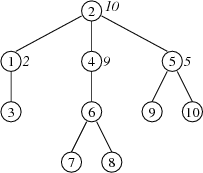
\includegraphics[]{pen.png}
\end{problem}

